\documentclass[11pt]{article}
% teacher_preamble.tex — shared preamble for the chalk-teaching TEACHER'S NOTES.
% These are standalone, instructor-facing lesson plans (article class), separate
% from the student lecture notes.  Compile each teaching/lecNN_teacher_notes.tex
% directly with pdfLaTeX.
\usepackage[T1]{fontenc}
\usepackage[utf8]{inputenc}
\usepackage[margin=1in]{geometry}
\usepackage{amsmath,amssymb,amsthm,mathtools}
\usepackage{braket}
\usepackage{bm}
\usepackage{graphicx}
\usepackage{enumitem}
\usepackage{xcolor}
\usepackage{tikz}
\usetikzlibrary{arrows.meta}
\usepackage{quantikz}
\usepackage[most]{tcolorbox}
\usepackage[colorlinks=true,linkcolor=blue,urlcolor=blue]{hyperref}

% ---- Notation macros (consistent with the course preamble.tex) ----
\newcommand{\R}{\mathbb{R}}
\newcommand{\C}{\mathbb{C}}
\newcommand{\N}{\mathbb{N}}
\newcommand{\Z}{\mathbb{Z}}
\newcommand{\E}{\mathbb{E}}
\newcommand{\Prob}{\mathbb{P}}
\newcommand{\Hilb}{\mathcal{H}}
\newcommand{\ii}{\mathrm{i}}
\newcommand{\dd}{\mathrm{d}}
\newcommand{\ee}{\mathrm{e}}
\DeclareMathOperator{\tr}{tr}
\DeclareMathOperator{\Tr}{Tr}
\DeclareMathOperator{\Var}{Var}
\DeclareMathOperator{\diag}{diag}
\newcommand{\norm}[1]{\left\lVert #1 \right\rVert}
\newcommand{\abs}[1]{\left\lvert #1 \right\rvert}
\newcommand{\bigo}{\mathcal{O}}
\newcommand{\id}{\mathbb{I}}
\newcommand{\dg}{^{\dagger}}
% quantikz also defines \proj (a circuit element we do not use); override it with our projector.
\let\proj\relax
\newcommand{\proj}[1]{\ket{#1}\!\bra{#1}}
\newcommand{\Xgate}{\mathsf{X}}
\newcommand{\Ygate}{\mathsf{Y}}
\newcommand{\Zgate}{\mathsf{Z}}
\newcommand{\Hgate}{\mathsf{H}}
\newcommand{\CNOT}{\mathrm{CNOT}}
\newcommand{\Uf}{U_f}

% ---- Theorem-like environments (numbered per section, article style) ----
\theoremstyle{definition}
\newtheorem{definition}{Definition}[section]
\newtheorem{example}[definition]{Example}
\theoremstyle{plain}
\newtheorem{theorem}[definition]{Theorem}
\newtheorem{lemma}[definition]{Lemma}
\newtheorem{proposition}[definition]{Proposition}
\theoremstyle{remark}
\newtheorem{remark}[definition]{Remark}

% ---- Teaching-specific structure ----
% Session block header with a time budget, e.g. \block{Qubits and the Bloch sphere}{45}
\newcommand{\block}[2]{%
  \bigskip\noindent
  \begin{tcolorbox}[colback=blue!6,colframe=blue!55!black,boxrule=0.6pt,arc=2pt,
    left=8pt,right=8pt,top=5pt,bottom=5pt]
  \textbf{\large #1}\hfill\textbf{[\,#2\,min]}
  \end{tcolorbox}}

% Board-plan cue: what to write/draw on the board.
\newtcolorbox{board}{colback=gray!8,colframe=gray!55!black,title={On the board},
  fonttitle=\bfseries\small,boxrule=0.5pt,arc=2pt,left=6pt,right=6pt,top=3pt,bottom=3pt}

% Graphic-demonstration cue (what to sketch).
\newcommand{\sketch}[1]{\par\smallskip\noindent{\color{teal}\textbf{Sketch:}} #1\par\smallskip}

% Optional / advanced material that may be skipped (but indicated).
\newtcolorbox{advanced}{colback=orange!7,colframe=orange!65!black,
  title={Advanced --- may be skipped (mention only)},
  fonttitle=\bfseries\small,boxrule=0.5pt,arc=2pt,left=6pt,right=6pt,top=3pt,bottom=3pt}

% Timing hint inline, e.g. \tmark{10} for a ~10-minute chunk.
\newcommand{\tmark}[1]{{\small\color{blue!55!black}(\,$\approx$#1\,min)}}

% In-class problem (numbered per section) and a teacher-facing answer.
\newtheorem{inclass}[definition]{In-class problem}
\newenvironment{answer}{\par\smallskip\noindent\textit{Answer.}\ }{\par\smallskip}

\title{\textbf{Lecture 1 --- Quantum Computation Basics}\\[0.3em]\large Teacher's Notes (chalk, one 3$\times$45\,min meeting)}
\author{Course Instructor}
\date{}
\begin{document}
\maketitle

\noindent\textbf{How to use these notes.} This is a chalk-delivery lesson plan for
one three-hour meeting, split into three 45-minute blocks. Boxed \textsf{On the
board} panels give the exact equations and text to write; \textcolor{teal}{\textbf{Sketch}}
cues say what to draw; \tmark{n} markers pace each chunk. Work the derivations
\emph{live} at the board rather than reading them out. Each block has in-class
problems with teacher-facing answers---put the problem up, give students 3--6
minutes, then walk the solution. Orange \emph{Advanced} boxes are optional; mention
them only if time allows.

\medskip
\noindent\textbf{Learning goals (by the end of the meeting a student can):}
\begin{itemize}[leftmargin=1.4em,nosep]
  \item Write a qubit as a unit vector in $\C^2$, apply the Born rule, and place a state on the Bloch sphere.
  \item Build multi-qubit states with tensor products, apply the standard gates $X,Y,Z,H,\CNOT$, and read a small circuit.
  \item Recognize entanglement (Bell state) and prove a two-qubit state is or is not separable.
  \item Prepare a target single-qubit state with $R_y,R_z$; measure in a rotated basis; state and prove no-cloning.
\end{itemize}

\medskip
\noindent\textbf{Prerequisites.} Linear algebra over $\C$ (inner products, unitary
matrices, eigenvectors), basic probability. No prior quantum computing assumed.

\medskip
\noindent\textbf{Materials.} Blackboard with room for a persistent
notation/gate ``cheat strip'' on one side; \emph{colored chalk} (white for algebra,
one color for measurement outcomes/probabilities, one for the Bloch sphere axes).

% =====================================================================
\block{Block 1 --- Qubits, superposition, and measurement}{45}
% =====================================================================
\noindent\emph{Objective:} a qubit is a unit vector in $\C^2$; the Born rule turns
amplitudes into probabilities; global phase is invisible; every state is a point on
the Bloch sphere.

\medskip
\noindent\textbf{Pacing:} Dirac notation \& the qubit \tmark{10}; Born rule \& phase
\tmark{10}; in-class problem 1 \tmark{6}; Bloch derivation \& sketch \tmark{13};
in-class problem 2 \tmark{6}.

\subsection*{1. Dirac notation and the single qubit \tmark{10}}
Open by fixing notation on the ``cheat strip'' and leaving it up all lecture.

\begin{board}
Ket = column vector, bra = conjugate-transpose row:
\[
  \ket{0}=\begin{pmatrix}1\\0\end{pmatrix},\quad
  \ket{1}=\begin{pmatrix}0\\1\end{pmatrix},\qquad
  \braket{x|y}=x\dg y=\sum_i \overline{x_i}\,y_i .
\]
Orthonormal basis: $\braket{i|j}=\delta_{ij}$; amplitude $=$ overlap $\braket{j|\psi}$.
\textbf{Qubit:} $\ket{\psi}=a\ket0+b\ket1$, $a,b\in\C$, $\abs{a}^2+\abs{b}^2=1$.
\end{board}

Stress the one postulate everything rests on: \emph{a state is a unit vector in a
complex Hilbert space}, and superposition is just closure under linear combination.

\subsection*{2. The Born rule; global vs.\ relative phase \tmark{10}}
\begin{board}
\textbf{Born rule.} Measuring $\ket{\psi}=a\ket0+b\ket1$ in the computational basis:
\[
  \Prob(0)=\abs{\braket{0|\psi}}^2=\abs{a}^2,\quad
  \Prob(1)=\abs{b}^2,\quad \text{state collapses to }\ket{0}\text{ or }\ket{1}.
\]
\textbf{Global phase invisible:} $\ee^{\ii\gamma}\ket{\psi}$ gives the same $\abs{a}^2,\abs{b}^2$.
\textbf{Relative phase is physical:}
$\ket{+}=\tfrac1{\sqrt2}(\ket0+\ket1)$ vs.\ $\ket{-}=\tfrac1{\sqrt2}(\ket0-\ket1)$,
same $z$-statistics but $\braket{+|-}=0$.
\end{board}

Emphasize the moral: probabilities see only \emph{moduli}, so an overall phase drops
out, but the \emph{relative} phase between $\ket0$ and $\ket1$ drives interference and
is measurable in a rotated basis (foreshadow Block 3).

\begin{inclass}[Normalize and read off probabilities]\label{ic:norm}
A qubit is $\ket{\psi}=2\ket0+\ii\ket1$ (unnormalized). Normalize it, then give
$\Prob(0)$ and $\Prob(1)$ in a computational-basis measurement.
\end{inclass}
\begin{answer}
$\norm{\psi}^2=\abs2^2+\abs{\ii}^2=4+1=5$, so
$\ket{\psi}=\tfrac1{\sqrt5}(2\ket0+\ii\ket1)$. Then
$\Prob(0)=\abs{2/\sqrt5}^2=4/5$ and $\Prob(1)=\abs{\ii/\sqrt5}^2=1/5$; they sum to $1$. \checkmark
\end{answer}

\subsection*{3. The Bloch sphere: derive the parametrization \tmark{13}}
Derive the Bloch form live---this is the geometric payoff of the block.

\begin{board}
\textbf{Claim.} Up to global phase every qubit is
\[
  \ket{\psi}=\cos\tfrac{\theta}{2}\ket0+\ee^{\ii\varphi}\sin\tfrac{\theta}{2}\ket1,
  \quad \theta\in[0,\pi],\ \varphi\in[0,2\pi).
\]
\textbf{Derivation.} Write $a=r_a\ee^{\ii\alpha}$, $b=r_b\ee^{\ii\beta}$, $r_a,r_b\ge0$.
Normalization $r_a^2+r_b^2=1$ $\Rightarrow$ set $r_a=\cos\tfrac\theta2$, $r_b=\sin\tfrac\theta2$.
Factor out $\ee^{\ii\alpha}$ (global phase, discard); put $\varphi=\beta-\alpha$.
\end{board}

\sketch{Bloch sphere: draw a circle with vertical axis $z$ (up $=\ket0$ at
$\theta{=}0$, down $=\ket1$ at $\theta{=}\pi$), horizontal $x$ axis
($\ket{\pm}=\tfrac1{\sqrt2}(\ket0\pm\ket1)$ front/back on equator), and $y$ axis
($\ket{\pm\ii}=\tfrac1{\sqrt2}(\ket0\pm\ii\ket1)$ left/right on equator). Mark angles
$\theta$ from $+z$ and $\varphi$ around the equator. \emph{Say aloud:} orthogonal
states are \emph{antipodal} ($\theta{=}\pi$ apart), not perpendicular.}

\begin{board}
\textbf{Landmarks:}\quad
$\ket0:\theta{=}0$;\ \ $\ket1:\theta{=}\pi$;\ \
$\ket{+}:(\tfrac\pi2,0)$;\ \ $\ket{-}:(\tfrac\pi2,\pi)$;\ \
$\ket{+\ii}:(\tfrac\pi2,\tfrac\pi2)$;\ \ $\ket{-\ii}:(\tfrac\pi2,\tfrac{3\pi}2)$.
\end{board}

\noindent Reference plot to reproduce on the board (state $\ket\psi$ at polar angle
$\theta$, azimuth $\varphi$), with the $z$-basis measurement shown as the projection
of the Bloch vector onto the $z$-axis:
\begin{center}
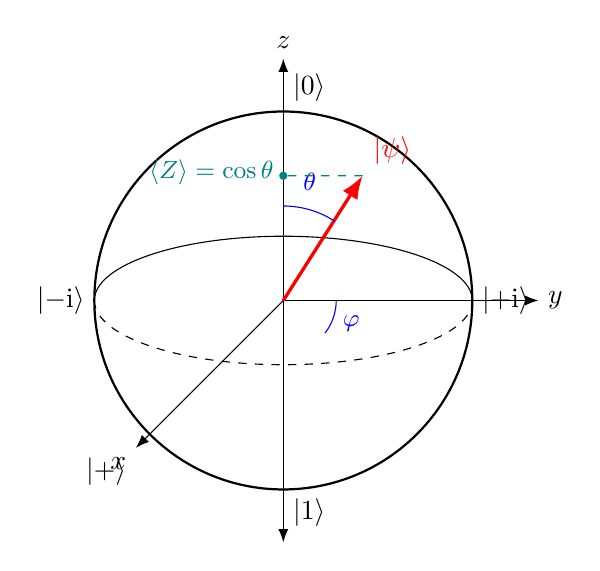
\begin{tikzpicture}[scale=2.4,>=Latex]
  \draw[thick] (0,0) circle (1);
  \draw[dashed] (-1,0) arc (180:360:1 and 0.34);
  \draw (1,0) arc (0:180:1 and 0.34);
  % axes
  \draw[->] (0,0) -- (0,1.28) node[above] {$z$};
  \draw[->] (0,0) -- (0,-1.28);
  \draw[->] (0,0) -- (1.35,0) node[right] {$y$};
  \draw[->] (0,0) -- (-0.78,-0.78) node[below left] {$x$};
  % landmarks
  \node[above right] at (0,1) {$\ket0$};
  \node[below right] at (0,-1) {$\ket1$};
  \node[right] at (1,0) {$\ket{+\ii}$};
  \node[left] at (-1,0) {$\ket{-\ii}$};
  \node[below left] at (-0.78,-0.78) {$\ket{+}$};
  % state vector at polar theta from +z, azimuth phi
  \coordinate (P) at (0.42,0.66);
  \draw[->,very thick,red] (0,0) -- (P) node[above right] {$\ket\psi$};
  % theta arc
  \draw[blue] (0,0.5) arc (90:57:0.5);
  \node[blue] at (0.14,0.63) {\small$\theta$};
  % azimuth phi arc near origin in the equatorial plane (schematic)
  \draw[blue] (0.28,0) arc (0:-38:0.28);
  \node[blue] at (0.36,-0.12) {\small$\varphi$};
  % z-basis measurement projection
  \draw[dashed,teal] (P) -- (0,0.66);
  \fill[teal] (0,0.66) circle (0.022);
  \node[teal,left] at (0,0.68) {\small $\langle Z\rangle=\cos\theta$};
\end{tikzpicture}
\end{center}

\begin{board}
\textbf{Measurement on the sphere.} A $z$-basis (computational) measurement of
$\ket{\psi(\theta,\varphi)}$ projects onto the poles:
\[
  \Prob(0)=\cos^2\tfrac\theta2=\tfrac{1+\cos\theta}{2},\quad
  \Prob(1)=\sin^2\tfrac\theta2=\tfrac{1-\cos\theta}{2},\quad
  \langle Z\rangle=\Prob(0)-\Prob(1)=\cos\theta .
\]
The azimuth $\varphi$ (relative phase) does \emph{not} affect $z$-statistics---you must
rotate first to see it (Block 3, ``measuring in a rotated basis'').
\end{board}

\begin{inclass}[Find the Bloch angles]\label{ic:bloch}
Give the Bloch angles $(\theta,\varphi)$ of $\ket{\psi}=\tfrac12\ket0+\tfrac{\sqrt3}{2}\ket1$
and of $\ket{+\ii}=\tfrac1{\sqrt2}(\ket0+\ii\ket1)$.
\end{inclass}
\begin{answer}
For the first: $\cos\tfrac\theta2=\tfrac12\Rightarrow\tfrac\theta2=\tfrac\pi3
\Rightarrow\theta=\tfrac{2\pi}3$; amplitudes real positive so $\varphi=0$. Check
$\sin\tfrac\theta2=\sin\tfrac\pi3=\tfrac{\sqrt3}2$. \checkmark\ \ For $\ket{+\ii}$:
equal moduli $\Rightarrow\theta=\tfrac\pi2$; relative phase $\ii=\ee^{\ii\pi/2}
\Rightarrow\varphi=\tfrac\pi2$.
\end{answer}

\begin{advanced}
Mixed states / density operators $\rho=\sum_i p_i\proj{\psi_i}$ live \emph{inside} the
Bloch ball ($\norm{\vec r}<1$); the center is the maximally mixed $\tfrac12\id$.
Deferred to Lecture 2. Mention only.
\end{advanced}

% =====================================================================
\block{Block 2 --- Multi-qubit systems, gates, and entanglement}{45}
% =====================================================================
\noindent\emph{Objective:} tensor products give a $2^n$-dimensional space; the
standard gates act by simple matrices; $H$ then $\CNOT$ builds an entangled Bell pair,
which we prove cannot factor.

\medskip
\noindent\textbf{Pacing:} tensor products \tmark{10}; single-qubit gates \tmark{9};
$\CNOT$ \& circuits \tmark{8}; Bell build + entanglement proof \tmark{12};
in-class problems interleaved \tmark{6}.

\subsection*{1. Tensor products and the $2^n$-dimensional space \tmark{10}}
\begin{board}
Composite system: $\Hilb_A\otimes\Hilb_B$, basis $\{\ket i_A\otimes\ket j_B\}$,
$\dim=(\dim\Hilb_A)(\dim\Hilb_B)$.
Shorthand $\ket i\otimes\ket j=\ket{ij}$. For $n$ qubits:
$\Hilb=(\C^2)^{\otimes n}\cong\C^{2^n}$, basis $\{\ket x:x\in\{0,1\}^n\}$.
Inner product factors: $(\bra i\otimes\bra j)(\ket k\otimes\ket l)=\braket{i|k}\braket{j|l}$.
\end{board}
Drive home the punchline: $n=50$ qubits $\Rightarrow 2^{50}>10^{15}$ amplitudes---a
classical description is exponentially large. This is the root of quantum power.

\begin{board}
\textbf{Separable vs.\ entangled.} $\ket\psi$ is a \emph{product state} if
$\ket\psi=\ket\alpha_A\otimes\ket\beta_B$; otherwise \emph{entangled}.
Two-qubit general state: $\ket\psi=\sum_{i,j}x_{ij}\ket{ij}$.
\end{board}

\subsection*{2. Single-qubit gates \tmark{9}}
A gate is a unitary ($U\dg U=\id$): preserves norm and inner products, hence reversible.

\begin{board}
\[
  X=\begin{pmatrix}0&1\\1&0\end{pmatrix},\
  Y=\begin{pmatrix}0&-\ii\\\ii&0\end{pmatrix},\
  Z=\begin{pmatrix}1&0\\0&-1\end{pmatrix},\
  H=\tfrac1{\sqrt2}\begin{pmatrix}1&1\\1&-1\end{pmatrix}.
\]
Action: $X\ket0=\ket1$ (bit flip); $Z\ket1=-\ket1$ (phase flip);
$H\ket0=\ket{+}$, $H\ket1=\ket{-}$; $H^2=\id$.
\end{board}

\noindent Circuit view --- a single wire carries the qubit, a box is a gate; e.g.\ $H$ on $\ket0$:
\begin{center}
\begin{quantikz}
\lstick{$\ket0$} & \gate{H} & \rstick{$\ket{+}$}\qw
\end{quantikz}
\end{center}
tying the picture to the algebra $H\binom{1}{0}=\tfrac1{\sqrt2}\binom{1}{1}$.

\begin{inclass}[Apply $H$ then measure]\label{ic:Hmeas}
Start in $\ket1$. Apply $H$, then measure in the computational basis. What state
results, and what are $\Prob(0),\Prob(1)$?
\end{inclass}
\begin{answer}
$H\ket1=\ket{-}=\tfrac1{\sqrt2}(\ket0-\ket1)$. Then $\Prob(0)=\abs{1/\sqrt2}^2=\tfrac12$
and $\Prob(1)=\tfrac12$; the $-$ sign (relative phase) does not affect
computational-basis probabilities.
\end{answer}

\noindent Circuit for this problem ($H$, then a computational-basis meter):
\begin{center}
\begin{quantikz}
\lstick{$\ket1$} & \gate{H} & \meter{} & \cw
\end{quantikz}
\end{center}

\subsection*{3. The $\CNOT$ and reading circuits \tmark{8}}
\begin{board}
\[
  \CNOT\ket{a,b}=\ket{a,\,a\oplus b},\qquad
  \CNOT=\begin{pmatrix}1&0&0&0\\0&1&0&0\\0&0&0&1\\0&0&1&0\end{pmatrix}
  \ \text{(basis } \ket{00}\ket{01}\ket{10}\ket{11}).
\]
Circuit reading: (1) time flows left$\to$right; (2) $\bullet$ = control (fires on
$\ket1$); (3) matrix order is \emph{reversed}: $U_1$ then $U_2$ $\Rightarrow U=U_2U_1$.
\end{board}

\noindent The Bell-state circuit --- $H$ on the top wire, then $\CNOT$ with control
$\bullet$ (top) and target $\oplus$ (bottom):
\begin{center}
\begin{quantikz}
\lstick{$\ket0$} & \gate{H} & \ctrl{1} & \qw \\
\lstick{$\ket0$} & \qw & \targ{} & \rstick[2]{$\ket{\Phi^+}$}\qw
\end{quantikz}
\end{center}

\subsection*{4. Build the Bell state; prove it is entangled \tmark{12}}
\begin{board}
\textbf{Bell build.} $\CNOT\,(H\otimes I)\ket{00}$:
\[
  (H\otimes I)\ket{00}=\tfrac1{\sqrt2}(\ket{00}+\ket{10})
  \ \xrightarrow{\ \CNOT\ }\ \tfrac1{\sqrt2}(\ket{00}+\ket{11})=\ket{\Phi^+}.
\]
\textbf{Entangled (coefficient matching).} Suppose $\ket{\Phi^+}=\ket\alpha\otimes\ket\beta$
with $\ket\alpha=a_0\ket0+a_1\ket1$, $\ket\beta=b_0\ket0+b_1\ket1$:
\[
  a_0b_0=\tfrac1{\sqrt2},\ \ a_0b_1=0,\ \ a_1b_0=0,\ \ a_1b_1=\tfrac1{\sqrt2}.
\]
$a_0b_0\ne0\Rightarrow a_0,b_0\ne0$; then $a_0b_1=0\Rightarrow b_1=0$ and
$a_1b_0=0\Rightarrow a_1=0$, so $a_1b_1=0\ne\tfrac1{\sqrt2}$. Contradiction.
\end{board}

\begin{inclass}[Separable or entangled?]\label{ic:sep}
Is $\ket\psi=\tfrac12(\ket{00}+\ket{01}+\ket{10}+\ket{11})$ entangled? If separable,
give the factorization.
\end{inclass}
\begin{answer}
Separable: $\ket\psi=\tfrac1{\sqrt2}(\ket0+\ket1)\otimes\tfrac1{\sqrt2}(\ket0+\ket1)
=\ket{+}\otimes\ket{+}$. Check by expanding: the four cross terms each carry $\tfrac12$. \checkmark
(Contrast with $\ket{\Phi^+}$, which has \emph{no} $\ket{01},\ket{10}$ terms and cannot factor.)
\end{answer}

\begin{advanced}
\textbf{CHSH / Bell nonlocality} (optional deep-dive, $\approx$10\,min if time allows).
Two parties share $\ket{\Phi^+}$; each picks one of two $\pm1$-valued measurements.
Form $S=A_1(B_1-B_2)+A_2(B_1+B_2)$.
\emph{Classical bound (realism+locality):} if $A_i,B_j\in\{\pm1\}$ all have definite
values, one of $B_1\mp B_2$ is $0$ and the other $\pm2$, so $S=\pm2$ each run and
$\abs{\E[S]}\le2$.
\emph{Quantum:} measuring $\ket{\Phi^+}$ along Bloch angles $\alpha,\beta$ gives
$\E[AB]=\cos(\alpha-\beta)$; at $\alpha_1{=}0,\alpha_2{=}\tfrac\pi2,\ \beta_1{=}\tfrac\pi4,
\beta_2{=}\tfrac{3\pi}4$,
$\E[S]=4\cos\tfrac\pi4=2\sqrt2\approx2.83>2$ (Tsirelson). Nature agrees with quantum
mechanics---no local-realistic model can. Full derivation in the student notes / Lecture 2.
\end{advanced}

% =====================================================================
\block{Block 3 --- Preparation, measurement, and no-cloning}{45}
% =====================================================================
\noindent\emph{Objective:} synthesize a target state with $R_y,R_z$; measure in a
rotated basis; state and prove the no-cloning theorem; close with a teleportation
teaser.

\medskip
\noindent\textbf{Pacing:} state prep from $\ket{0\cdots0}$ \tmark{12}; measuring in a
rotated basis \tmark{10}; no-cloning proof \tmark{10}; teleportation capstone
\tmark{7}; in-class problems interleaved \tmark{6}.

\subsection*{1. Preparing states from $\ket{0\cdots0}$ \tmark{12}}
\begin{board}
\textbf{Cheap prep.} Basis state $\ket x$: apply $X$ to each qubit with $x_j=1$ ($\le n$ gates).
Uniform superposition: $H^{\otimes n}\ket{0\cdots0}=\dfrac1{\sqrt{2^n}}\sum_{x}\ket x$ ($n$ gates).
\textbf{Single-qubit synthesis} of $\ket{\psi(\theta,\varphi)}=\cos\tfrac\theta2\ket0+\ee^{\ii\varphi}\sin\tfrac\theta2\ket1$:
\[
  R_y(\theta)=\begin{pmatrix}\cos\tfrac\theta2&-\sin\tfrac\theta2\\[2pt]\sin\tfrac\theta2&\cos\tfrac\theta2\end{pmatrix},\quad
  R_z(\varphi)=\begin{pmatrix}\ee^{-\ii\varphi/2}&0\\0&\ee^{\ii\varphi/2}\end{pmatrix},
\]
and $R_z(\varphi)R_y(\theta)\ket0=\ee^{-\ii\varphi/2}\ket{\psi(\theta,\varphi)}$ (global phase, drop).
\end{board}
Interpretation: $R_y$ tips the Bloch vector down by $\theta$ (sets moduli); $R_z$
spins it by $\varphi$ around the axis (sets relative phase).

\begin{center}
\begin{quantikz}
\lstick{$\ket0$} & \gate{R_y(\theta)} & \gate{R_z(\varphi)} & \rstick{$\ket{\psi(\theta,\varphi)}$}\qw
\end{quantikz}
\end{center}

\begin{inclass}[Give the preparation angles]\label{ic:prep}
Which $R_y(\theta)$, $R_z(\varphi)$ prepare $\ket{+\ii}=\tfrac1{\sqrt2}(\ket0+\ii\ket1)$
from $\ket0$? Give one single-gate alternative.
\end{inclass}
\begin{answer}
From In-class~\ref{ic:bloch}, $\ket{+\ii}$ has $\theta=\tfrac\pi2$, $\varphi=\tfrac\pi2$.
So $R_z(\tfrac\pi2)R_y(\tfrac\pi2)\ket0$: $R_y(\tfrac\pi2)\ket0=\ket{+}$, then
$R_z(\tfrac\pi2)$ adds relative phase $\ee^{\ii\pi/2}=\ii$. Single-gate alternative:
$S\ket{+}=\ket{+\ii}$ (so $S\,H\ket0$), since $S=\diag(1,\ii)$.
\end{answer}

\begin{advanced}
General amplitude encoding of an arbitrary $n$-qubit state costs $\bigo(2^n)$ gates in
the worst case (matching an $\Omega(2^n)$ lower bound); structured states (product,
sparse, efficiently-computable) are cheaper. Deferred to Lecture 6. Mention only.
\end{advanced}

\subsection*{2. Measuring in a rotated basis \tmark{10}}
\begin{board}
Hardware measures in the $z$ basis only. To measure basis $\{\ket{\phi_m}\}$ apply
$V$ with $V\ket{\phi_m}=\ket m$, then measure:
$\abs{\braket{\phi_m|\psi}}^2=\abs{\braket{m|V|\psi}}^2$.
\textbf{$X$ basis:} $V=H$ since $H\ket{+}=\ket0$, $H\ket{-}=\ket1$.
So ``measure $X$'' $=$ apply $H$, then measure $z$; read $\ket{+}\!\to\!0$, $\ket{-}\!\to\!1$.
Expectation: $\langle O\rangle=\bra{\psi}O\ket{\psi}$.
\end{board}

\begin{board}
\textbf{Why ``measure $X$'' $=$ apply $H$ then measure $Z$} (derive on the board):
\begin{enumerate}[leftmargin=1.5em,itemsep=1pt,topsep=2pt]
  \item \emph{What $X$ means.} $X=(+1)\proj{+}+(-1)\proj{-}$, so measuring $X$ \emph{is}
        the projective measurement in its eigenbasis $\{\ket{+},\ket{-}\}$ (outcome $\pm1$).
  \item \emph{Basis change.} To measure in a basis $\{\ket{\phi_m}\}$, apply $V$ with
        $V\ket{\phi_m}=\ket m$, then measure $z$:
        $\Prob(m)=\abs{\braket{m|V|\psi}}^2=\abs{\braket{\phi_m|\psi}}^2$ (using $\bra m V=\bra{\phi_m}$).
  \item \emph{$H$ is that $V$.} $H\ket{+}=\ket0,\ H\ket{-}=\ket1$ (and $H=H\dg$, $H^2=\id$),
        so reading $\ket0\!\to\!+1$, $\ket1\!\to\!-1$ reproduces the $X$-statistics:
        $\Prob(+1)=\abs{\braket{+|\psi}}^2=\abs{\braket{0|H|\psi}}^2$.
\end{enumerate}
\emph{One line:} $H$ \emph{diagonalizes} $X$, i.e.\ $HXH=Z$; conjugating the observable by
$H$ turns an $X$-measurement into a $Z$-measurement. (Likewise $V=H S\dg$ gives a $Y$-measurement,
since $Y$'s eigenbasis is $\ket{\pm\ii}$.)
\end{board}

\noindent Circuit --- ``measure $X$'' is $H$ followed by a computational-basis meter:
\begin{center}
\begin{quantikz}
\lstick{$\ket\psi$} & \gate{H} & \meter{$Z$} & \cw
\end{quantikz}
\end{center}

\noindent Picture: an $X$-basis measurement projects the Bloch vector onto the
$x$-axis (the $\ket{\pm}$ poles of the rotated basis); equivalently, $H$ rotates the
$x$-axis onto the $z$-axis and we read the meter as usual.
\begin{center}
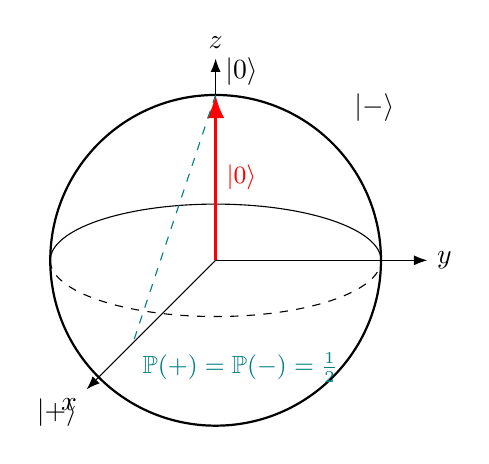
\begin{tikzpicture}[scale=2.1,>=Latex]
  \draw[thick] (0,0) circle (1);
  \draw[dashed] (-1,0) arc (180:360:1 and 0.34);
  \draw (1,0) arc (0:180:1 and 0.34);
  \draw[->] (0,0) -- (0,1.22) node[above] {$z$};
  \draw[->] (0,0) -- (1.28,0) node[right] {$y$};
  \draw[->] (0,0) -- (-0.78,-0.78) node[below left] {$x$};
  \node[above right] at (0,1) {$\ket0$};
  \node[below left] at (-0.78,-0.78) {$\ket{+}$};
  \node[above right] at (0.78,0.78) {$\ket{-}$};
  % state |0> on +z, projected onto the x-axis (the +/- measurement axis)
  \draw[->,very thick,red] (0,0) -- (0,1) node[midway,right] {\small$\ket0$};
  \draw[dashed,teal] (0,1) -- (-0.5,-0.5);
  \node[teal,below right] at (-0.5,-0.5) {\small $\Prob(+)=\Prob(-)=\tfrac12$};
\end{tikzpicture}
\end{center}

\begin{inclass}[Measurement in the $X$ basis]\label{ic:xbasis}
For $\ket0$, find $\Prob(+)$ and $\Prob(-)$ in the $X$ basis and $\langle X\rangle$.
Then do the same for $\ket{+}$.
\end{inclass}
\begin{answer}
$\braket{+|0}=\tfrac1{\sqrt2}$, $\braket{-|0}=\tfrac1{\sqrt2}$, so
$\Prob(+)=\Prob(-)=\tfrac12$ and $\langle X\rangle=\tfrac12(+1)+\tfrac12(-1)=0$
(equivalently apply $H$ to $\ket0$ giving $\ket{+}$, then $z$-measure: $50/50$).
For $\ket{+}$: it \emph{is} the $+1$ eigenstate, so $\Prob(+)=1$, $\Prob(-)=0$,
$\langle X\rangle=1$. Complementarity: $\ket{+}$ is sharp in $X$ but maximally
uncertain in $Z$.
\end{answer}

\subsection*{3. The no-cloning theorem \tmark{10}}
\begin{board}
\textbf{No-cloning.} There is no unitary $U$ and blank $\ket s$ with
$U(\ket\psi\otimes\ket s)=\ket\psi\otimes\ket\psi$ for \emph{all} $\ket\psi$
(when $\dim\Hilb\ge2$).
\textbf{Proof.} Apply to $\ket{x_1},\ket{x_2}$ and take inner products.
Left (unitary, $\braket{s|s}=1$): $\braket{x_1|x_2}$.
Right (tensor factors): $\braket{x_1|x_2}^2$. So with $z=\braket{x_1|x_2}$,
\[
  z=z^2\ \Rightarrow\ z\in\{0,1\}.
\]
But e.g.\ $\braket{0|+}=\tfrac1{\sqrt2}\notin\{0,1\}$. Contradiction. $\square$
\end{board}
One-line moral to say aloud: cloning $\ket\psi\mapsto\ket\psi\otimes\ket\psi$ is
\emph{quadratic} in $\ket\psi$, but gates are \emph{linear}---linearity forbids it.

\begin{inclass}[$\CNOT$ does not clone]\label{ic:cnotclone}
Show $\CNOT$ does not copy the superposition $\ket x=a\ket0+b\ket1$: compute
$\CNOT(\ket x\otimes\ket0)$ and compare with $\ket x\otimes\ket x$.
\end{inclass}
\begin{answer}
$\CNOT(\ket x\ket0)=a\ket{00}+b\ket{11}$, whereas
$\ket x\ket x=a^2\ket{00}+ab\ket{01}+ab\ket{10}+b^2\ket{11}$. They differ unless
$ab=0$ (i.e.\ $\ket x$ is a basis state): the cross terms $ab\ket{01},ab\ket{10}$ are
missing on the left. $\CNOT$ copies only classical (basis) information.
\end{answer}

\subsection*{4. Capstone: teleportation teaser \tmark{7}}
Tie the meeting together: entanglement (Block 2) $+$ measurement (Block 3) $+$
no-cloning $\Rightarrow$ you can \emph{move} an unknown qubit, not copy it.
\emph{Motivating story (Brody, Ch.~4):} Penelope teleports a qubit across the Aegean to
the seafaring Odysseus, using an entangled pair they made \emph{before} parting.

\begin{board}
\textbf{Teleportation (sketch).} Penelope has unknown $\ket\psi$ (qubit 1) and half of
$\ket{\Phi^+}$ (qubit 2); Odysseus holds qubit 3. Penelope applies $\CNOT_{1\to2}$, then $H_1$,
measures $(m_1,m_2)$ (each of 4 outcomes, prob.\ $\tfrac14$). Odysseus's qubit is then
$X^{m_2}Z^{m_1}\ket\psi$; he applies $Z^{m_1}X^{m_2}$ to recover $\ket\psi$.
Needs 2 classical bits; source is destroyed (no-cloning safe); no signaling.
\end{board}

\noindent The teleportation circuit --- the left $H,\CNOT$ on wires 2--3 create
$\ket{\Phi^+}$; then $\CNOT_{1\to2}$, $H_1$, the two meters, and the feed-forward
corrections $X^{m_2},Z^{m_1}$ on Odysseus's wire (switched on by the classical outcomes):
\begin{center}
\begin{quantikz}
\lstick{$\ket\psi$} & \qw      & \qw      & \ctrl{1} & \gate{H} & \meter{} & \cw & \cw \\
\lstick{$\ket0$}    & \gate{H} & \ctrl{1} & \targ{}  & \qw      & \meter{} & \cw & \cw \\
\lstick{$\ket0$}    & \qw      & \targ{}  & \qw      & \qw      & \qw      & \gate{X^{m_2}} & \gate{Z^{m_1}}\rstick{$\ket\psi$}
\end{quantikz}
\end{center}

\begin{board}
\textbf{Why it works (amplitude tracking --- do it live).} Let $\ket\psi=a\ket0+b\ket1$;
order the qubits $(1,2,3)$. Start from $\ket\psi\otimes\ket{\Phi^+}$:
\[
  \tfrac1{\sqrt2}\big[a\ket0(\ket{00}+\ket{11})+b\ket1(\ket{00}+\ket{11})\big].
\]
Apply $\CNOT_{1\to2}$ (flip qubit 2 when qubit 1 is $\ket1$), then $H_1$:
\[
  \xrightarrow{\ \CNOT_{1\to2}\ }
  \tfrac1{\sqrt2}\big[a\ket0(\ket{00}+\ket{11})+b\ket1(\ket{10}+\ket{01})\big]
\]
\[
  \xrightarrow{\ H_1\ }\tfrac12\big[\,
  \ket{00}(a\ket0+b\ket1)+\ket{01}(a\ket1+b\ket0)
  +\ket{10}(a\ket0-b\ket1)+\ket{11}(a\ket1-b\ket0)\,\big].
\]
Group by Penelope's two bits $(m_1,m_2)$ (each outcome equally likely, prob.\ $\tfrac14$):
Odysseus's qubit 3 is left in $X^{m_2}Z^{m_1}\ket\psi$:
\[
  (0,0)\!\to\!\ket\psi,\quad (0,1)\!\to\! X\ket\psi,\quad
  (1,0)\!\to\! Z\ket\psi,\quad (1,1)\!\to\! XZ\ket\psi,
\]
so Odysseus applies $Z^{m_1}X^{m_2}$ to recover $\ket\psi$ exactly.
\end{board}

\noindent\textbf{What this teaches (say aloud):}
\begin{itemize}[leftmargin=1.5em,itemsep=1pt,topsep=2pt]
  \item \emph{Resources:} one shared Bell pair (entanglement) $+$ two classical bits move one
        unknown qubit. Entanglement alone cannot; classical bits alone cannot.
  \item \emph{No-cloning respected:} Penelope's measurement collapses qubits 1--2, destroying her
        copy---the state is \emph{moved}, not duplicated. The amplitudes $a,b$ are never learned.
  \item \emph{No faster-than-light signaling:} before the two bits arrive, Odysseus's four branches are
        equally likely, so his qubit is the maximally mixed $\tfrac12\id$---he learns nothing until
        the classical message is received.
  \item \emph{Information, not matter:} only quantum \emph{information} (the amplitudes $a,b$)
        crosses the gap---rebuilt on Odysseus's pre-existing qubit from 2 classical bits $+$ shared
        entanglement; no qubit or mass travels (Brody, Ch.~4).
\end{itemize}

\begin{inclass}[One correction branch]\label{ic:tele}
In teleportation, suppose Penelope measures $(m_1,m_2)=(1,0)$. What is Odysseus's qubit before
correction, and which gate(s) fix it?
\end{inclass}
\begin{answer}
Odysseus holds $X^{0}Z^{1}\ket\psi=Z\ket\psi=a\ket0-b\ket1$. Since $m_1=1,m_2=0$ he applies
$Z^{1}X^{0}=Z$; because $Z^2=\id$, $Z(Z\ket\psi)=\ket\psi$. \checkmark
\end{answer}

\subsection*{5. Superdense coding --- the dual (optional / extension) \tmark{6}}
The same Bell resource run ``in reverse'': send \emph{two} classical bits by
transmitting \emph{one} qubit.
\begin{board}
Penelope and Odysseus share $\ket{\Phi^+}$ (qubit 1 Penelope's, qubit 2 Odysseus's).
To send $(x,y)\in\{0,1\}^2$, Penelope applies $Z^{x}X^{y}$ to \emph{her} qubit and sends
it over; the four choices map $\ket{\Phi^+}$ to the four orthonormal Bell states:
\[
  (0,0)\!:\tfrac1{\sqrt2}(\ket{00}+\ket{11}),\quad
  (0,1)\!:\tfrac1{\sqrt2}(\ket{10}+\ket{01}),
\]
\[
  (1,0)\!:\tfrac1{\sqrt2}(\ket{00}-\ket{11}),\quad
  (1,1)\!:\tfrac1{\sqrt2}(\ket{10}-\ket{01}).
\]
Odysseus applies $\CNOT_{1\to2}$ then $H_1$ (the inverse Bell circuit) and measures,
reading $(x,y)$ with certainty.
\end{board}
\noindent\emph{Duality:} 1 qubit $+$ 1 shared Bell pair $\leftrightarrow$ 2 classical
bits; teleportation and superdense coding are the two directions of the same trade.
\begin{center}
\begin{quantikz}
\lstick{$\ket0$} & \gate{H} & \ctrl{1} & \gate{Z^{x}X^{y}} & \ctrl{1} & \gate{H} & \meter{} \\
\lstick{$\ket0$} & \qw & \targ{} & \qw & \targ{} & \qw & \meter{}
\end{quantikz}
\end{center}

\begin{inclass}[Encode two bits]\label{ic:superdense}
Which gate does Penelope apply to send $(x,y)=(1,1)$, and which Bell state results?
\end{inclass}
\begin{answer}
$Z^{1}X^{1}=ZX$ on her qubit: $X\otimes\id$ takes $\ket{\Phi^+}$ to
$\tfrac1{\sqrt2}(\ket{10}+\ket{01})$, then $Z\otimes\id$ to
$\tfrac1{\sqrt2}(\ket{01}-\ket{10})$ (the singlet, up to global phase). Odysseus's
inverse Bell circuit then returns $\ket{11}$, i.e.\ $(1,1)$. \checkmark
\end{answer}

\begin{advanced}
\textbf{Bridge to Lecture 2 --- density operators} (optional; the natural sequel).
When we hold only \emph{part} of an entangled pair, or a probabilistic mixture, a single
ket no longer suffices: use $\rho=\sum_i p_i\proj{\psi_i}$ with $\Tr\rho=1$,
$\rho\succeq0$. Born rule becomes $p(m)=\Tr[P_m\rho]$, $\langle M\rangle=\Tr[M\rho]$.
\emph{Pure} iff $\Tr[\rho^2]=1$, else \emph{mixed}; the maximally mixed $\tfrac12\id$
has $\Tr[\rho^2]=\tfrac12$. The \emph{reduced state} of one half of $\ket{\Phi^+}$ is
$\rho_A=\Tr_B\proj{\Phi^+}=\tfrac12\id$---exactly why Odysseus's teleportation marginal
is $\tfrac12\id$ and no-signaling holds. POVMs / Naimark dilation, shot-noise
$M=\bigo(1/\varepsilon^2)$, and complexity classes are also set up in the student notes
and taken up in Lecture 2.
\end{advanced}

\end{document}
